\chapter{NetFI-3}
NetFi-3 es una actualización de un trabajo previo~\cite{netfi2} el cual, a partir de un re-diseño original de NetFi~\cite{6555963} se obtuvo una metodología con la cual se podía realizar inyección de fallos a nivel RTL. Dicho método si bien demostró ser eficiente a nivel hardware (puesto que ya no era necesario de hardware adicional a la FPGA donde se realizaban las pruebas de inyección), dejaba demasiados cabos sueltos en su contraparte de software, debido a la inmensa curva de aprendisaje requerida para implementar siquiera el diseño más simple bajo NetFi-2.

Este trabajo entonces logra convertir lo que una vez era una metodología, a lo que es ahora, un completo suite de herramientas automatizadas que nos permiten no solo realizar inyecciones de forma eficiente, rápida y con la seguridad requerida al momento de trabajar con diseños RTL, sino también nos brinda un total y completo control sobre como realizar dichas inyecciones, obtención de resultados. Por último, pero no menos importante, las herramientas ahora implementadas cumplen con la ventaja de ser extensibles de una manera mucho más fácil, no solo por la extensa y precisa documentación elaborada, sino por la descentralización de componentes reutilizables de software implementados.

El núcleo central y más importante de este trabajo es la re arquitectura realizada a MODNET, su migración a python y nuevo caracter de implementación, el cual nos permite automatizar un flujo de inyección de fallos con una simple CLI (command line interface)

\section{MODNET v2}
MODify NETlist (MODNET) es una herramienta desarrollada por Wassim Mansou para su tesis doctoral en el laboratorio TIMA. El software fue diseñado para tomar una Netlist de un circuito a  someter, realizándole cambios en los lugares que se consideran sensibles, para que la inyección de fallos sea posible. 

Uno de los problemas más grandes de este software es su falta de capacidad para ser automatizable dentro de un flujo completo de NetFI. Además de esto, MODNET se desarrollo en lenguaje C\#, el cual, para ser compilado depende por completo de la herramienta Visual Studio 2012, la cual es privativa y de uso bajo licencia, convirtiendo al software en uno de los componentes más problematicos del sistema.

En este trabajo se tomó la funcionalidad central de MODNET y se realizó una ingeniería inversa de su código para obtener así las claves necesarias para implementarla en cualquier lenguaje. El objetivo con esto no es solo el poder hacer cambios grandes en la arquitectura general del funcionamiento del software en si, pero además para poder documentar extensivamente sus funcionalidades y de esta manera poder extender en el futuro sus capacidades para poder realizar inyecciones en cualquier tipo de Netlist (desde una de Vivado, hasta una del software open-source de síntesis de FPGA YOSIS)
	\subsection{Arquitectura de MODNET}
	Al momento de escribir este informe, el código HDL del circuito a someter se puede sintetizar mediante la herramienta Synplify Premier únicamente. Con esta herramienta se escoge para que tipo de tecnología se desea sintetizar el código HDL, la misma genera la Netlist en Verilog del DUT. La Netlist así generada se sitúa en la entrada de MODNET para automatizar el proceso de modificación de las bibliotecas del Xilinx. Algunos de los componentes modificados son los FFD y sus distintos ejemplares (FDC, FDE, etc.) y también las LUTs que incluye las compuertas lógicas y los multiplexores.
La salida de MODNET es la Netlist modificada con  señales extras de entradas usadas para inyectar las fallas en los registros y las compuertas lógicas. De esta manera se logra preparar un RTL para que puedan inyectarse SEUs y SETs. En este sentido, la arquitectura interna original no se cambia y se respeta tal cual es. 


\subsection{Emulación de SEU: Flip-Flops}
En la figura ~\ref{FF} se muestra el extra hardware que se debe agregar para generar un circuito capaz de ser implementado para un futuro proceso de inyecciones. Se puede notar que el extra hardware se limita a un multiplexor, la señal de inyección INJ y una compuerta NOR.
En la figura ~\ref{FFS} se puede ver su comportamiento y cómo  actua en el caso que haya una inyección o en el caso que no la haya. Se muestra que su comportamiento original no se modifica en el caso en que la inyección  no suceda. Es por ello que el cambio es no invasivo y respecta el comportamiento original del circuito.


\begin{figure}[H]
	\centering
	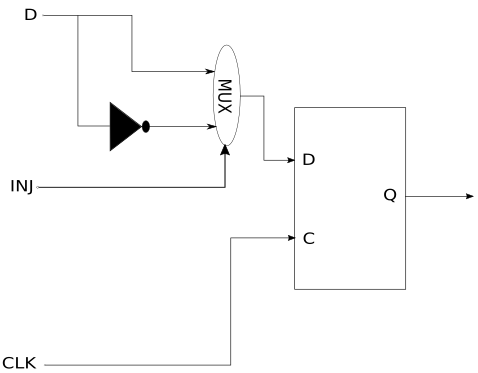
\includegraphics[width=0.55 \textwidth]{img/FF.png}
	\caption{Modificación de un Flip-Flop sin la señal de habilitación}
	\label{FF}
\end{figure}

\begin{figure}[H]
	\centering
	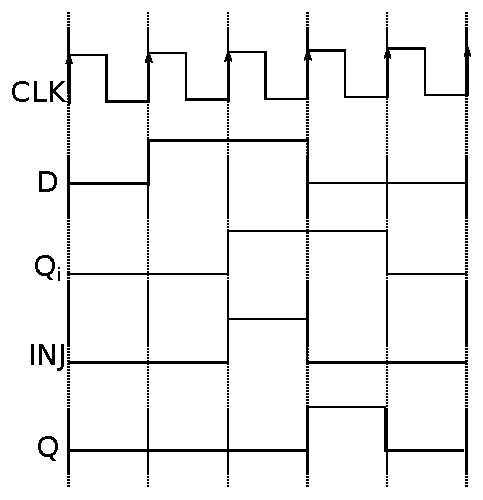
\includegraphics[width=0.48 \textwidth]{img/dessin.pdf}
	\caption{Formas de la onda del FF modificada con  $Q_{i}$ la cual es la salida original sin INJ }
	\label{FFS}
\end{figure}

En la siguiente fracción de  código se puede ver la traducción final en la biblioteca modificada de Xilinx.
\lstset{frame=tb,
  language=VHDL,
  aboveskip=3mm,
  belowskip=3mm,
  showstringspaces=false,
  columns=flexible,
  basicstyle=\ttfamily,
  numbers=none,
  breakatwhitespace=true,
  tabsize=2
}

\begin{lstlisting}

module FDC_mod (inj, Q, C, CLR, D);

parameter INIT = 1'b0;

output Q;

input C, CLR, D, inj;

wire Din;

FDC uut_FDC(.Q(Q),.C(C),.CLR(CLR),.D(Din));

assign Din = (inj) ? !D : D;

endmodule

\end{lstlisting}

Es necesario  aclarar que existen diferentes tipos de modificaciones posibles en los flip-flop las cuales se asemejan más a la realidad dependiendo del tipo de circuito. Podríamos hacer una primera clasificación sobre los FF en FF que se leen, FF que  se escriben o en FF que hacen las dos cosas. Dependiendo del funcionamiento del circuito se utilizará un tipo u otro FF. De esta forma, la biblioteca que define el comportamiento del FF en Xilinx se remplaza por su versión modificada. Ya que puede ser crítico el momento en que llega la señal de inyección, esto puede ocurrir mientras se está escribiendo el circuito o mientras se está leyendo, pudiendo ocasionar un cambio o no. Por ejemplo, si nuestro circuito solo usa FFD sin \textit{enable}, solo nos interesarán las inyecciones en la escritura del FF, pero si fuese un FFDE el cual pose un \textit{enable}, podría ocurrir que se lea  el FFDE y simultáneamente cayese una inyección, quedando el FFDE en un estado inestable, este tipo de problemas se solucionan con  más lógica combinacional, por lo tanto, más hardware extra.

En la figura ~\ref{FFDE} se muestra la descripción esquemática de un FFDE con su lazo para volver  a un estado estable y el extra hardware para el proceso de inyeccion. El FFDE estará activo cuando la suma de INJ y CE sean iguales a 1. Las opciones son  01 ó 10.  


\begin{figure}[H]
	\centering
	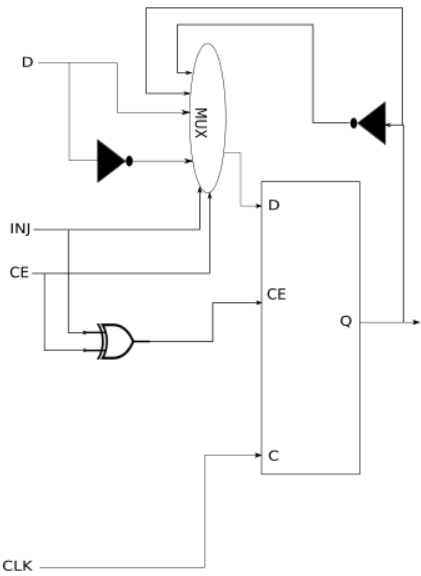
\includegraphics[width=0.5 \textwidth]{img/FFDE.png}
	\caption{Modificación de un FFDE }
	\label{FFDE}
\end{figure}

Por otro lado, en la figura ~\ref{FFDESS}  se puede ver que cuando los estados INJ  y CE son 00 ó 11 el FFDE  no se activa, manteniendo su salida Q.

\begin{figure}[H]
	\centering
	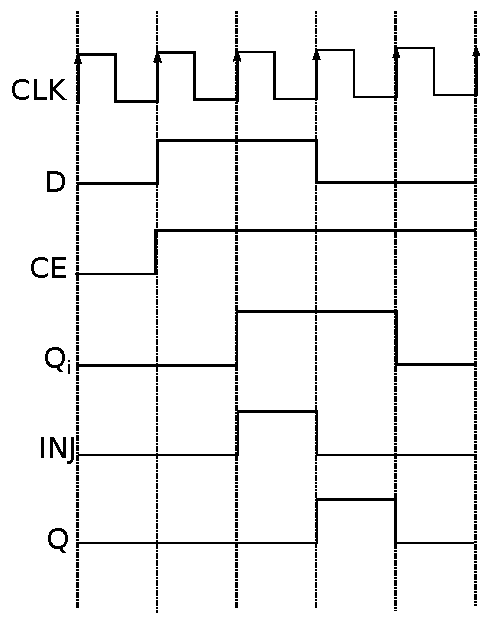
\includegraphics[width=0.4 \textwidth]{img/FFDES.pdf}
	\caption{Comportamiento de un FFDE  modificado }
	\label{FFDESS}
\end{figure}


\subsection{Emulación de SET: Look-Up Table }

Como se menciono anteriormente, luego  de la síntesis con  Synplify Pro, los circuitos  bajo prueba dan como resultado los siguientes tipos de LUTs: LUT4, LUT4\_L, LUT5, LUT5\_L,LUT6, LUT6\_L, a los cuales se le aplica las alteraciones pertinentes para que tengan efecto las futuras inyecciones, tal cual se muestra en la figura \ref{LUT}. En el Anexo A se encuentra el código completo de las librerías que se corresponden a las LUTs original y modificadas.


\begin{figure}[H]
	\centering
	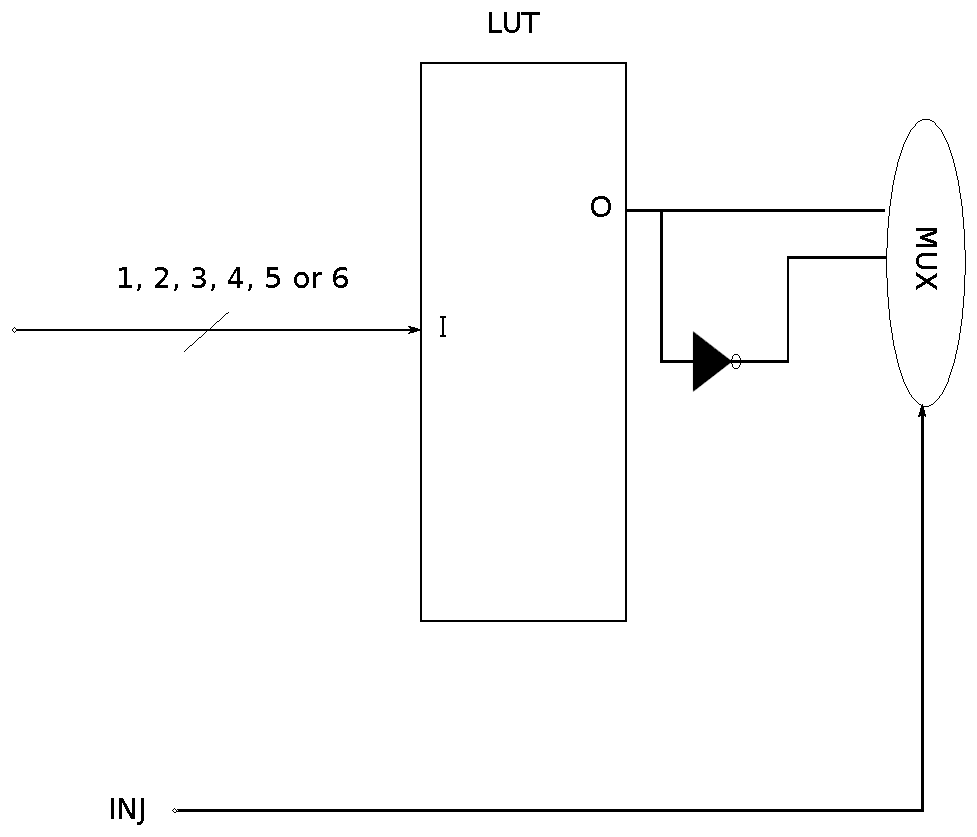
\includegraphics[width=0.4 \textwidth]{img/LUT.pdf}
	\caption{Modificación de una LUT}
	\label{LUT}
\end{figure}


Traducido a código una LUT, independientemente del tipo, a la biblioteca que la define solamente se le agrega  un multiplexor a la salida, el cual será controlado por una señal de inyección. 
\begin{lstlisting}
  module LUT6_L (inj_c,LO, I0, I1, I2, I3, I4, I5);

  parameter INIT = 64'h0000000000000000;

  input inj_c,I0, I1, I2, I3, I4, I5;

  output LO;

  reg LO1;
  reg tmp;
  
  assign LO = (!inj_c) ? LO1 : !LO1;
\end{lstlisting}

En el extracto de código anterior se intenta mostrar que independientemente de la arquitectura que tenga cada LUT, si ocurriese una falla, la salida será la negación del valor correcto de la LUT, determinada por la condición de decisión la cual se implementa en el circuito con un simple  multiplexor.

	\subsection{Descripción de MODNET v2}
	MODNET v2 es la segunda gran iteración de este software de inyección de fallos. Uno de los cambios más grandes es la migración de C\# a Python 3. Esto no solo abre el abanico de posibilidades de nuevas implementaciones de manera más sencilla, pero además es un lenguaje de libre uso, y al ser interpretado facilita al proyecto realizar cambios y validaciones de una manera en la cual antes simplemente era imaginable.

En esta migración se tomaron estrictas medidas de como se realizaría el código, como estaría estructurado y como extenderlo. Si bien su implementación actual sigue estando atada a NetLists realizadas por Synplify Premier, extenderlo es algo trivial. La lectura del código es mucho más sencilla y se encuentra documentado en su totalidad, de esta manera permitiendo a futuros trabajos en extender la herramienta y lograr así el crecimiento de un producto a su máximo potencial.

La totalidad del desarrollo se encuentra alojado en GitHub de manera pública, en los repositorios del LCSR. Y puede encontrarse en \href{https://github.com/LCSR-lab/MODNET}{https://github.com/LCSR-lab/MODNET}

La obtención de una NetList puede hacerse a través de un software de síntesis de FPGA. Como se mencionó, MODNET v2 actualmente soporta NetLists obtenidas desde Synplify Premier. Este paquete de soluciones es desarrollado por Synopsys Inc. una compañía estadounidense líder en el desarrollo de software especializado para el diseño de circuitos integrados complejos. La única desventaja de esto es que el software funciona bajo licencia, y desafortunadamente no ofrece una licencia de uso educativo universitario.

En la UNC contamos con licencia para utilizar este software y al LCSR se le brindó el acceso remoto a un servidor con el software instalado en su versión 2017, y es con el cual se describirá el proceso de obtención de una NetList.

El proceso entero será explicado a partir de un diseño de una máquina bayesiana diseñada en el laboratorio TIMA, el cual se conoce como "BM Slice". Además, la implementación fue realizada en una FPGA Nexys 4, por lo tanto la configuración específica del proyecto en cuanto al dispositivo se encuentra configurado para funcionar solo en la Nexys 4.
		\subsubsection{Obtención de una NetList}
		Synplify Premier cuenta con una funcionalidad "shell" como ellos la describen, que significa básicamente que el software puede correrse de la terminal sin la necesidad de una GUI (esto nos permite automatizar el proceso de síntesis).

Para obtener la NetList de un diseño RTL se necesitan 2 componentes: el primero, es un script que se ejecuta de forma remota y realiza la síntesis en si. El segundo es un script "tcl", que no es otra cosa que un lenguaje que Sinplify puede interpretar para realizar diferentes tareas. En el caso de la BM Slice, este script tiene la siguiente forma: \break


\begin{lstlisting}
    # Crea un proyecto nuevo en Sinplify
    project -new proyectos/bm_slice.prj

    # Guarda el proyecto
    project -save proyectos/bm_slice.prj

    # Agrega los componentes de la BM Slice 
    add_file -vhdl ./bm.vhd
    add_file -vhdl ./bm_slice.vhd
    add_file -vhdl ./params.vhd
    add_file -vhdl ./sto_add2.vhd
    add_file -vhdl ./sto_add3.vhd
    add_file -vhdl ./sto_mul2.vhd
    add_file -vhdl ./sto_mul3.vhd

    # Guardar netlist en formato verilog 
    set_option -result_file proyectos/rev_1/bm_slice.vm

    # Configuracion para Nexys 4
    set_option -technology ARTIX7
    set_option -part XC7A100T
    set_option -package CSG324
    set_option -grade -1

    # Comienzo de la sintesis
    project -run
    exit    
    
\end{lstlisting}

La salida de Synplify en \path{proyectos/rev_1/bm_slice.vm} es la NetList que necesitamos como entrada a MODNET v2
		\subsubsection{Desde las bases (migración a python3)}
		Uno de los desafíos más grandes en este proyecto era migrar el código de MODNET a python. Para comenzar, se le solicitó al laboratorio TIMA el código actual en C\# para comenzar su estudio.

Fue una sorpresa encontrarnos que el código estaba prácticamente abandonado desde el 2013 y no había una última versión clara, se encontró una versión en internet que se obtuvo desde la tesis en PDF de Wassim, y el resto del código original de lo provisto por el laboratorio que se encontraba en un disco externo en Francia.

Una vez con el código en mano, se decidió subir una primera release a GitHub del código original en C\#, para así preserver tanto el legado del doctor Wassim, como así también para facilitar el trabajo a desarrollar en la migración.

Una de las primeros bloqueos que se encontraron fue que el código de MODNET debía ser recompilado para cada DUT que se quisiera someter bajo prueba. Es decir, que para poder siquiera implementar un cambio mínimo en un diseño RTL, era necesario contar con la suite completa de Visual Studio 2012. Además, la ubicación de la NetList debía ser configurada en tiempo de compilación como se observa en la figura ~\ref{modnet_gui_1}, complicando aún más el uso de la herramienta.

\begin{figure}[H]
	\centering
	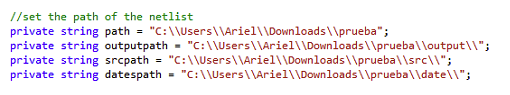
\includegraphics[width=1 \textwidth, frame]{img/modnet_gui_1.png}
	\caption{ Código original que solicitaba definir la ubicación de la NetList en tiempo de compilación}
	\label{modnet_gui_1}
\end{figure}

Por otra parte, el código original era muy complicado de interpretar y seguir. Se podían observar mucha cantidad de modificaciones de string sin ninguna explicación, como la inclusión de diversos caracteres que moficicaban el comportamiento del DUT sin siquiera un comentario de porque se realizaba. Como ejemplo, en la figura ~\ref{modnet_gui_5} se muestra el código que inserta una entrada de inyección de fallo si: 

\begin{enumerate}
    \item La línea contiene 2 caracteres especiales, un espacio en blanco y un paréntesis abierto,
    \item si la lógica es de tipo secuencial,
    \item si el tipo de error es SEU.
\end{enumerate}

\begin{figure}[H]
	\centering
	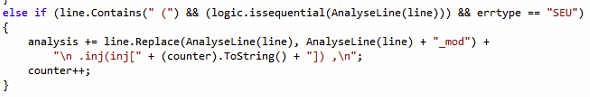
\includegraphics[width=\linewidth, frame ]{img/modnet_gui_5.png}
	\caption{ Insersión de un lugar a inyección de fallo por MODNET original}
	\label{modnet_gui_5}
\end{figure}

Esto no es solo confunso, sino que además imposibilita por completo a la extensión del proyecto. ¿Qué significa `` ('' ? ¿Es específico a la NetList de Synplify?. Estas son algunas de las preguntas que surgieron durante el desarrollo que se intentaron solucionar a partir de la implementación de clases en python, abstrayendo así al programador dentro de la lógica de inyección de fallas sobre como está elaborada la NetList, y asi acelerando el proceso de desarrollo.

Por otra parte, la implementación de MODNET requería de la interacción con una GUI, que se ve en la figura \ref{modnet_gui_4}. Es decir, que si se solucionaban algunos de los problemas anteriormente nombrados, aún se estaba atado a tener que lidiar con una interfaz gráfica que no permitiría la automatización del sistema.

\begin{figure}[H]
	\centering
	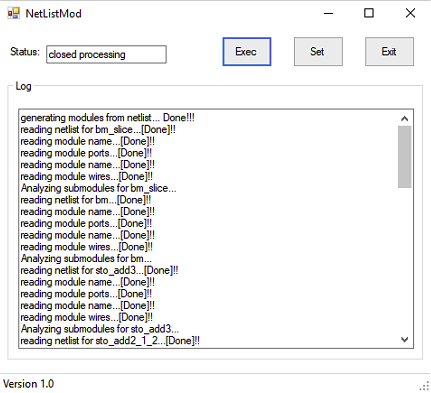
\includegraphics[width=0.6 \textwidth, frame]{img/modnet_gui_4.png}
	\caption{Ejecución de un proceso de inyección de lugares de falla en MODNET v1.}
	\label{modnet_gui_4}
\end{figure}

En la figura \ref{modnet_python_1} podemos observar la misma sección de código luego de ser traducida a python. En la misma se puede observar como `` ('' se convierte en un atributo de la clase \textit{ModuleCst} llamado \textit{COMPONENT\_START}, de esta manera queda claro que se comienza a iterar en busca de puntos sensibles de inyección a partir del comienzo de la declaración de un componente (por ejmplo, una LUT), haciendo el código más legible y fácil de seguir. Por otro lado, esto facilita la extensión de MODNET v2 hacia otro tipo de NetLists, ya que basta con definir un tipo de \textit{COMPONENT\_START} para cada netlist (como puede ser, una para Synplify y otro para Yosis), haciendo que la lógica que busca puntos sensibles no deba cambiar, simplemente se comportará de manera distinta dependiendo del tipo de NetList que se esté procesando.

\begin{figure}[H]
	\centering
	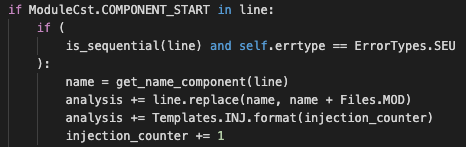
\includegraphics[width=0.8 \textwidth]{img/modnet_python_1.png}
	\caption{ Insersión de un lugar a inyección de fallo por MODNET v2}
	\label{modnet_python_1}
\end{figure}

Se puede observar además como el lugar de inyección ahora parte de un \textit{template} de la clae \textit{Templates}, en donde se define que una inyección para Synplify tiene el formato \path{inj[]}, pudiendo así extender para otras NetLists como debería representarse dentro de un componente el inicio de un punto sensible o lugar de inyección. Estos son solo algunas de las mejoras que se implmentarond de cara a la migración a Python 3. El seguimiento y esquema de release del proyecto se encuentran dentro del repositorio de GitHub donde se puede apreciar todas las etapas por las cuales se sometió a la implementación original.
		\subsubsection{Construcción de LUTs (transformación a LUT2)}
		Una LookUp Table, o LUT, en términos generales es básicamente una tabla que determina cuál es la salida para cualquier entrada dada. En el contexto de la lógica combinacional, es la tabla de verdad. Esta tabla de verdad define efectivamente cómo se comporta su lógica combinatoria.

En otras palabras, cualquier comportamiento que obtenga al interconectar cualquier número de compuertas (como AND, NOR, etc.), sin rutas de retroalimentación (para garantizar que no tenga estado), puede implementarse mediante una LUT.

Una LUT generalmente se construye a partir de Bits SRAM para contener la máscara LUT de la memoria de configuración (CRAM) y un conjunto de multiplexores para seleccionar el bit de CRAM que es conducido a la salida. Para implementar una LUT de entrada k (LUTk), una LUT que puede implementar cualquier función de k entradas necesita 2\textsuperscript{k} bits SRAM y un multiplexor 2\textsuperscript{k}:1. La Figura \ref{altera_luts_1} muestra una LUT4, que consta de 16 bits de SRAM y un multiplexor 16:1 implementado como un árbol de multiplexores 2:1. La LUT4 puede implementar cualquier función de 4 entradas (A, B, C, D) configurando el valor apropiado en la máscara LUT. Para simplificar la LUT4 en la Figura \ref{altera_luts_1}, también se puede construir a partir de dos LUT3 conectadas por un multiplexor 2:1.

\begin{figure}[H]
	\centering
	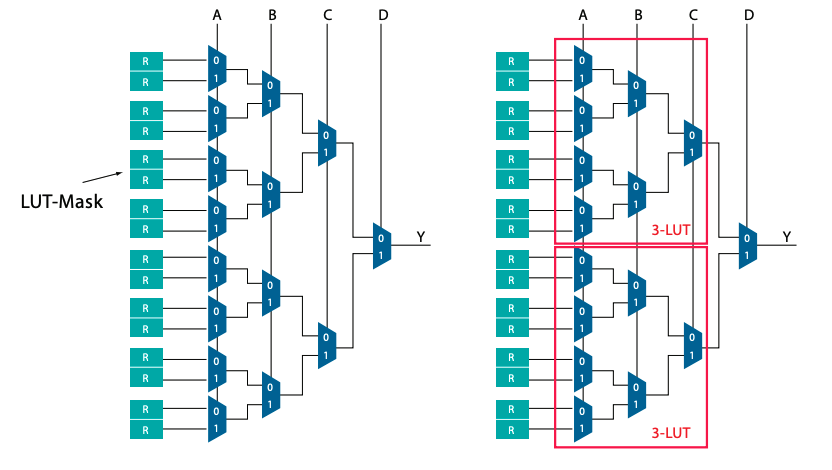
\includegraphics[width=1 \textwidth]{img/altera_luts_1.png}
	\caption{Construyendo una LUT}
	\label{altera_luts_1}
\end{figure}


De manera similar, las LUT más grandes se pueden construir a partir de las más pequeñas ~\cite{alteraLUTs}, como se muestra en la Figura \ref{altera_luts_2}. Por ejemplo, se puede construir una LUT5 con dos LUT4 y un multiplexor, mientras que un LUT6 se puede construir con dos LUT5 y un multiplexor. Técnicamente, lo importante es el número total de bits CRAM en la LUT y que se utilizan para implementar una función arbitraria de seis entradas.


\begin{figure}[H]
	\centering
	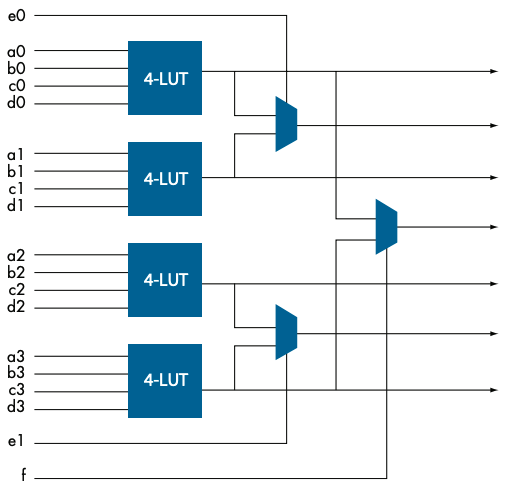
\includegraphics[width=0.6 \textwidth]{img/altera_luts_2.png}
	\caption{Composición de LUTs más grandes a partir de LUTs más pequeñas}
	\label{altera_luts_2}
\end{figure}

Teniendo esto en cuenta, y sabiendo que MODNET permite realizar una inyección por cada LUT dentro del circuito, podemos transformar de forma iterativa cada una de las LUTs existentes para convertirlas en LUT2, y así conseguir un aumento exponencial de inyecciones mayor al anteriormente conseguido, como se observa en la figura \ref{lut4_to_lut2}.

\begin{figure}[t]
	\centering
	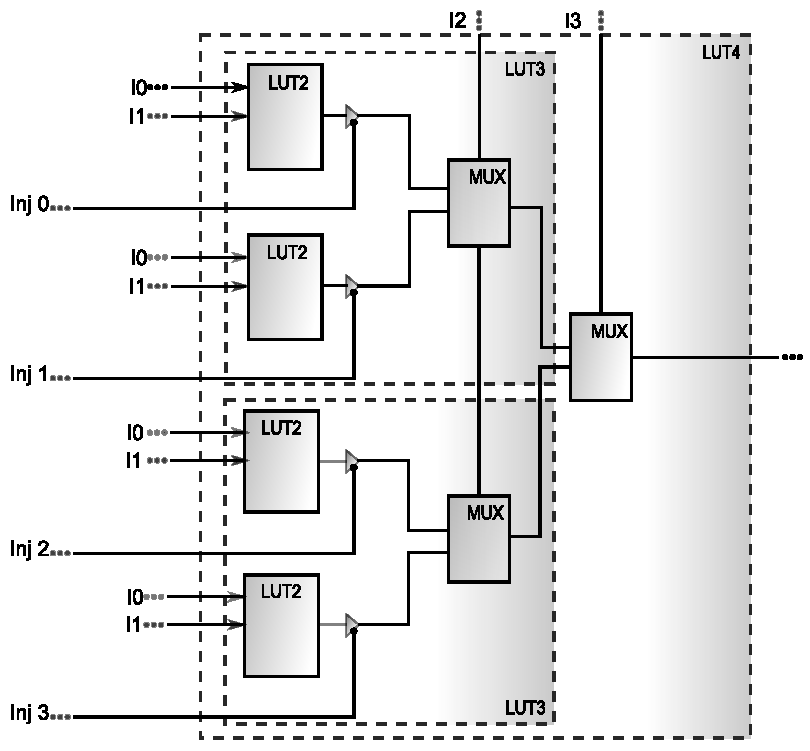
\includegraphics[width=0.7 \textwidth]{img/Lut4_IN_LUT2.pdf}
	\caption{Implementación de una a LUT4 con 4 LUT2s y 3 multiplexores o 2 LUT3s y 2 multiplexers}
	\label{lut4_to_lut2}
\end{figure}
		\subsubsection{Puesta en marcha}
		MODNET v2 cuenta con una CLI (command line interface), a diferencia de su predecesor. La herramienta se encuentra publicada en PyPI, por lo tanto su instalación es muy sencilla, simplemente corriendo:

\break

\begin{lstlisting}
    pip install mod-net
\end{lstlisting}

Para su utilización, y en su estado actual, MODNET necesita como entrada

\begin{itemize}
    \item Ubicación de la NetList a procesar,
    \item Nombre del módulo top del sistema,
    \item Directorio de salida (por defecto utiliza \path{ubicacion_de_la_netlist/output})
\end{itemize}

Entonces se corre el comando \emph{modnet} con sus parámetros:

\break

\begin{lstlisting}
    modnet --netlist ejemplo/netlist.vm --top-module top_module --outdir ./output
\end{lstlisting}

De esta manera MODNET creará un árbol de archivos con la salida correspondiente al siguiente esquema:

\begin{forest}
    for tree={
      font=\ttfamily,
      grow'=0,
      child anchor=west,
      parent anchor=south,
      anchor=west,
      calign=first,
      edge path={
        \noexpand\path [draw, \forestoption{edge}]
        (!u.south west) +(7.5pt,0) |- node[fill,inner sep=1.25pt] {} (.child anchor)\forestoption{edge label};
      },
      before typesetting nodes={
        if n=1
          {insert before={[,phantom]}}
          {}
      },
      fit=band,
      before computing xy={l=15pt},
    }
  [example
    [netlist.vm]
    [output
        [modulo1\_con\_iny.v]
        [modulo2\_con\_iny.v]
        [modulo3\_con\_iny.v]
    ]
    [src
        [modulo1.v]
        [modulo2.v]
    ]
  ]
  \end{forest}

El contenido de \path{output/} es lo que nos interesa, ya que es el resaultado de insertar las inyecciones a la NetList proveniente de Synplify Premier. En el próximo capitulo se procede a explicar como se integran todos los componentes de NetFI-3, y más importante, como conseguir una completa automatización de una campaña de inyecciones.


\section{Arquitectura de NetFI-3}
\input{content/arq_netfi.tex}
	\subsection{Microblaze}
	\input{content/microblaze.tex}
	\subsection{AXI4}
	\input{content/axi4.tex}
	\subsection{Integración de componentes}
	\input{content/integracion_de_componentes.tex}
	\subsection{Automatización del proceso de inyecciones}
	\input{content/automatizacion_inyecciones.tex}